\documentclass[11pt]{article}

\usepackage{amsmath, amssymb, amsthm}
\usepackage{tikz}

\theoremstyle{plain}
\newtheorem{thm}{Theorem}[section]
\newtheorem*{thm*}{Theorem}
\newtheorem{prop}[thm]{Proposition}
\newtheorem{lem}[thm]{Lemma}
\newtheorem*{lem*}{Lemma}
\newtheorem{dfn}[thm]{Definition}
\newtheorem{cor}[thm]{Corollary}
\newtheorem{claim}[thm]{Claim}
\newtheorem{conj}[thm]{Conjecture}
\newtheorem{ques}[thm]{Question}
\newtheorem*{rem}{Remark}


\oddsidemargin  0pt
\evensidemargin 0pt
\marginparwidth 40pt
\marginparsep 10pt
\topmargin 0pt
\headsep 10pt
\textheight 8.2in
\textwidth 6.4in
\renewcommand{\baselinestretch}{1.1}

\newcommand{\codeg}{\text{codeg}}
\newcommand{\BBE}{\mathbb{E}}
\newcommand{\BFP}{\mathbf{P}}
\usepackage{amsmath}
\usepackage{amsthm}
\usepackage{amssymb}
\usepackage{mathtools}
\usepackage{hyperref}
\usepackage{url}





\usepackage{graphicx}
\usepackage{caption}
\usepackage{subcaption}

\def\eQb#1\eQe{\begin{eqnarray*}#1\end{eqnarray*}}
\def\eQnb#1\eQne{\begin{eqnarray}#1\end{eqnarray}}
\providecommand{\e}[1]{\ensuremath{\times 10^{#1}}}
\providecommand{\pb}[0]{\pagebreak}
\DeclarePairedDelimiter\ceil{\lceil}{\rceil}
\DeclarePairedDelimiter\floor{\lfloor}{\rfloor}

\newcommand{\E}{\mathrm{E}}
\newcommand{\Var}{\mathrm{Var}}
\newcommand{\Cov}{\mathrm{Cov}}

\def\Qb#1\Qe{\begin{question}#1\end{question}}
\def\Sb#1\Se{\begin{solution}#1\end{solution}}


\newtheoremstyle{quest}{\topsep}{\topsep}{}{}{\bfseries}{}{ }{\thmname{#1}\thmnote{ #3}.}
\theoremstyle{quest}
\newtheorem*{definition}{Definition}
\newtheorem*{theorem}{Theorem}
\newtheorem*{lemma}{Lemma}
\newtheorem*{question}{Question}
\newtheorem*{preposition}{Preposition}
\newtheorem*{exercise}{Exercise}
\newtheorem*{challengeproblem}{Challenge Problem}
\newtheorem*{solution}{Solution}
\newtheorem*{remark}{Remark}
\usepackage{verbatimbox}
\usepackage{listings}
\usepackage{mathrsfs}
\date{}
\title{\vspace{-0.7cm}
Limit Theorems II: Final}

\author{
Youngduck Choi 
\thanks{Department of Mathematics, Courant Institute of Mathematical Sciences, 
yc1104@nyu.edu; If you find an error and want to share with me, 
you can reach me via email.
}}

\begin{document}

\maketitle

\begin{abstract}
This work contains solutions for the final of the Limit Theorems II by Professor
McKean.
\end{abstract}


\begin{question}[1-1]
\hfill
\begin{figure}[h!]
  \centering
    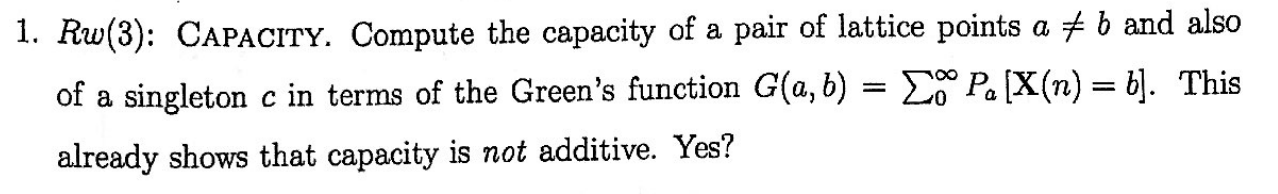
\includegraphics[width=0.7\textwidth]{limthm2-f-p1.png}
\end{figure}
\end{question}
\begin{solution} \hfill \\
\end{solution}

\newpage

\begin{question}[1-2]
\hfill
\begin{figure}[h!]
  \centering
    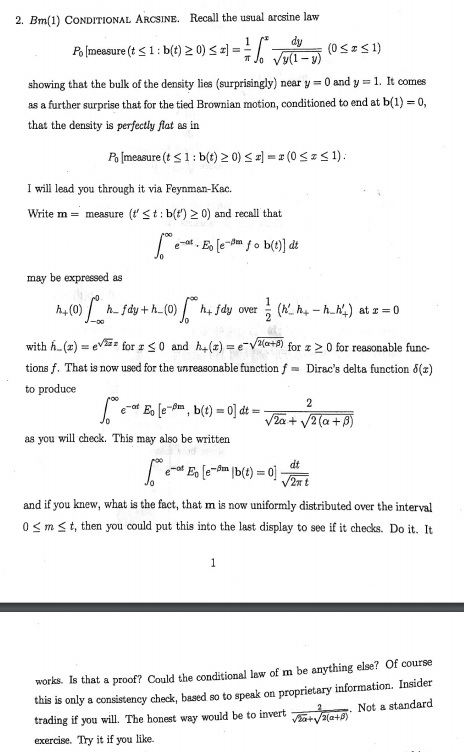
\includegraphics[width=0.7\textwidth]{limthm2-f-p2.png}
\end{figure}
\end{question}
\begin{solution} \hfill \\
\end{solution}

\newpage

\begin{question}[1-3]
\hfill
\begin{figure}[h!]
  \centering
    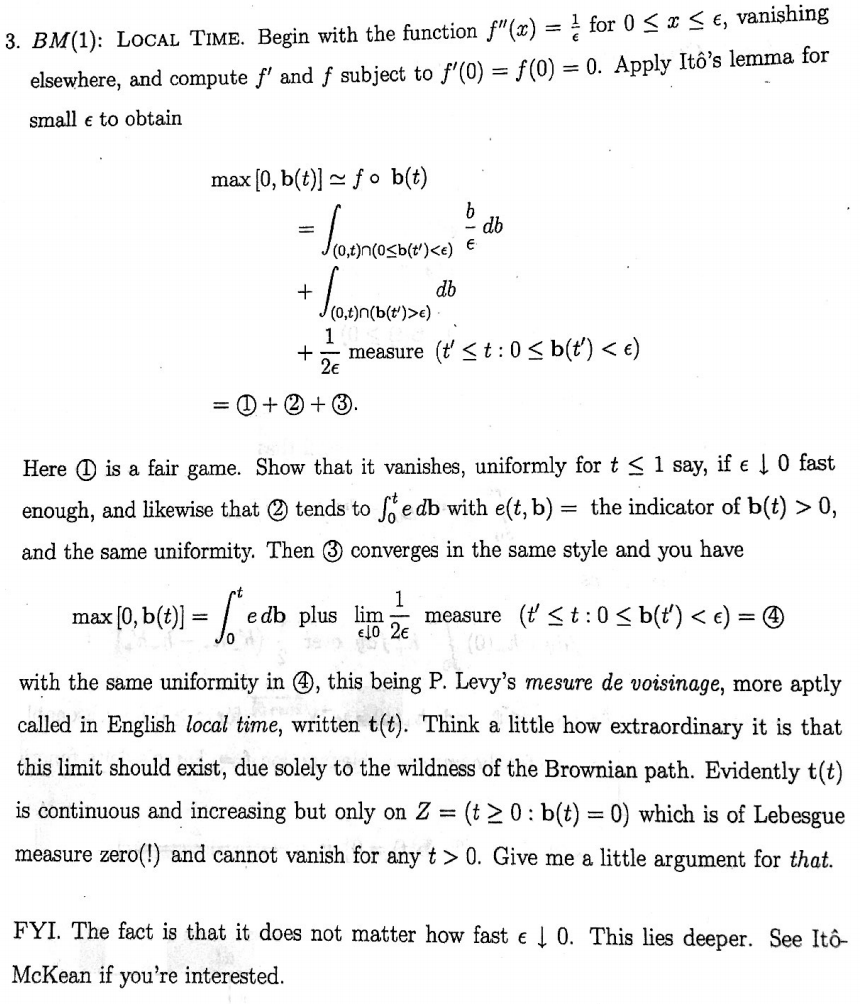
\includegraphics[width=0.7\textwidth]{limthm2-f-p3.png}
\end{figure}
\end{question}
\begin{solution} \hfill \\
Recall the Ito's formula for single martingales: If $f$ is $C^2$ and for all $0 \leq t$,
\eQb
E\int_{0}^{t} [f'(M(s))]^2 dA(s) < \infty \>\>\> &\text{and}& \>\>\> E\int_{0}^{t} 
|f''(M(s))|dA(s) < \infty
\eQe
then, for all $0 \leq t$,
\eQnb
f(M(t)) - f(M(0)) &=& \int_{0}^{t} f'(M(s)) dM(s) + \dfrac{1}{2} \int_{0}^{t} 
f'(M(s)) dA(s) \label{eq:1-3-1}
\eQne
where $A(t)$ is the unique increasing, continuous process, corresponding to $M(t)$.
Of course, for the problem at hand, we have $M(t) = B(t)$ and $A(t) = t$, so $db(s)$ and
$ds$ will be used to denote the integrators. 
Now, to compute local time, we cannot naively apply this formula, as $\max(0,\cdot)$ is 
not $C^2(\mathbb{R})$. Hence, we approximate with the suggested strategy. 
Let $f_{\epsilon}$ be defined as given for each $\epsilon > 0$. Then, 
for any $0 \leq t$, and $\epsilon > 0$,
\eQnb
f_{\epsilon} \circ b(t) &=& f_{\epsilon} \circ b(t) - f_{\epsilon} \circ b(0) 
= \int_{0}^{t} f_{\epsilon}^{'}(B(s)) db(s) + \dfrac{1}{2} \int_{0}^{t}  
f_{\epsilon}^{''} (B(s)) ds \label{eq:1-3-2} \\ 
&=& \int_{\{s \in [0,t] : 0 \leq b(s) < \epsilon\}} \dfrac{b(s) }{\epsilon} db(s)
+ \int_{\{s \in [0,t] : b(s) > \epsilon\}} 1 db(s)
+ \dfrac{1}{2} \int_{ \{s \in [0,t] : 0 \leq b(s) < \epsilon\} } \dfrac{1}{\epsilon} 
ds  \label{eq:1-3-3} \\
&=& 
\int_{\{s \in [0,t] : 0 \leq b(s) < \epsilon\}} \dfrac{b(s) }{\epsilon} db(s)
+ \int_{\{s \in [0,t] : b(s) > \epsilon\}} 1 db(s) \nonumber 
+ \dfrac{1}{2\epsilon} \lambda_1( \{ s \in [0,t] : 0 \leq b(s) < \epsilon \}) \nonumber
\\ 
&=:& (I) + (II) + (III) \nonumber 
\eQne 
where~\eqref{eq:1-3-2} follows from~\eqref{eq:1-3-1},~\eqref{eq:1-3-3} follows
from definition of $f_{\epsilon}$ for each $\epsilon > 0$, and $\lambda_1$ denotes
1-dimensional Lebesgue measure as hinted. With the given fact that $(I)$ is a 
martingale, we show that
\eQb
\int_{\{s \in [0,1] : 0 \leq b(s) < \epsilon\}} \dfrac{b(s)}{\epsilon} db(s) \>\> 
\text{converges to} 0  as \epsilon \to 0 \>\>\> \text{almost surely}  
\eQe 
dd
 
\end{solution}

\newpage

\begin{question}[1-4]
\hfill
\begin{figure}[h!]
  \centering
    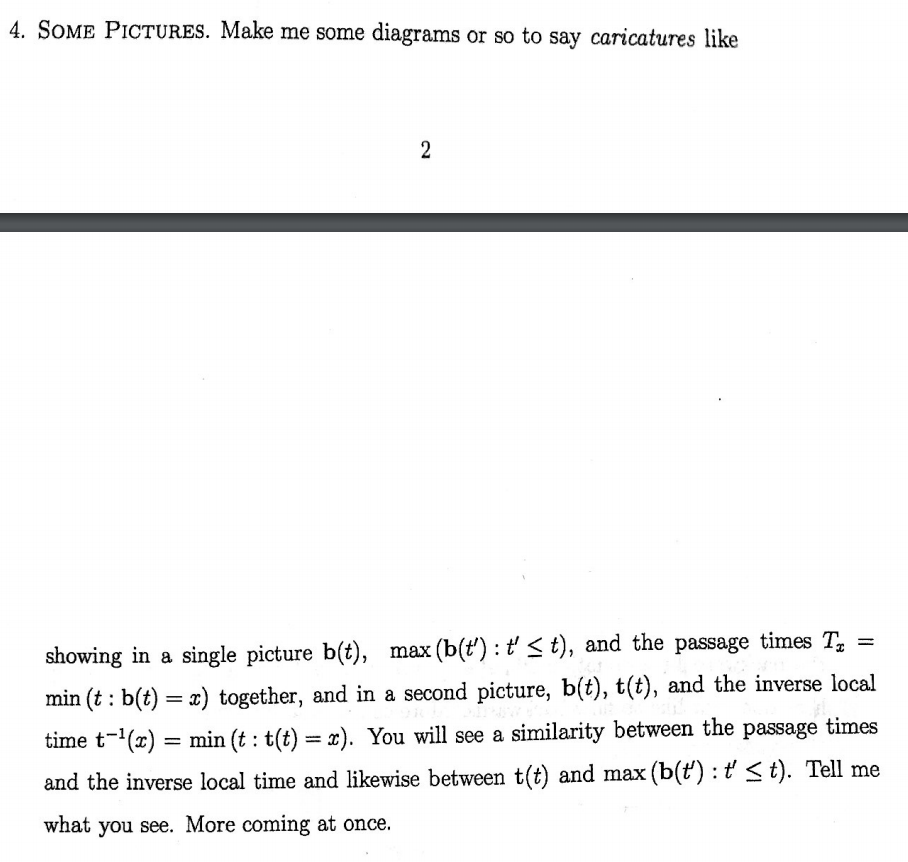
\includegraphics[width=0.7\textwidth]{limthm2-f-p4.png}
\end{figure}
\end{question}
\begin{solution} \hfill \\
\end{solution}

\newpage

\begin{question}[1-5]
\hfill
\begin{figure}[h!]
  \centering
    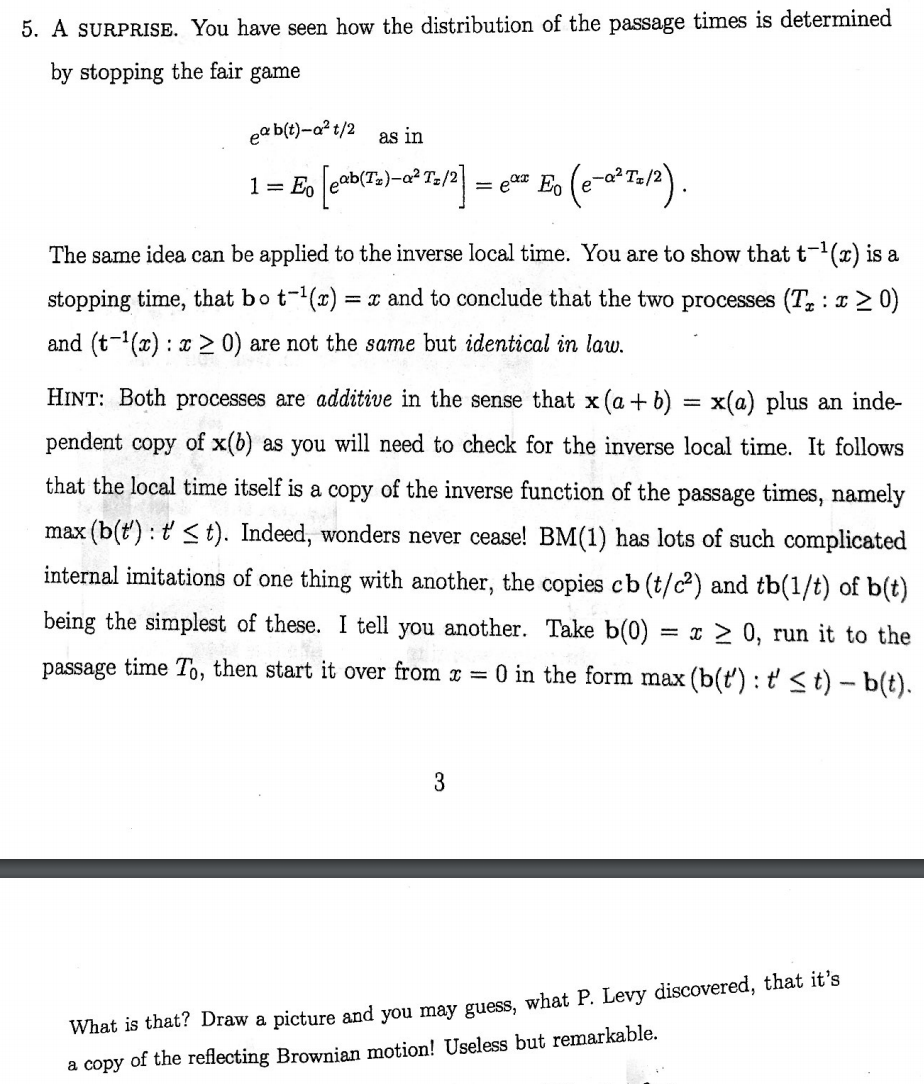
\includegraphics[width=0.7\textwidth]{limthm2-f-p5.png}
\end{figure}
\end{question}
\begin{solution} \hfill \\
\end{solution}

\newpage

\begin{question}[1-6]
\hfill
\begin{figure}[h!]
  \centering
    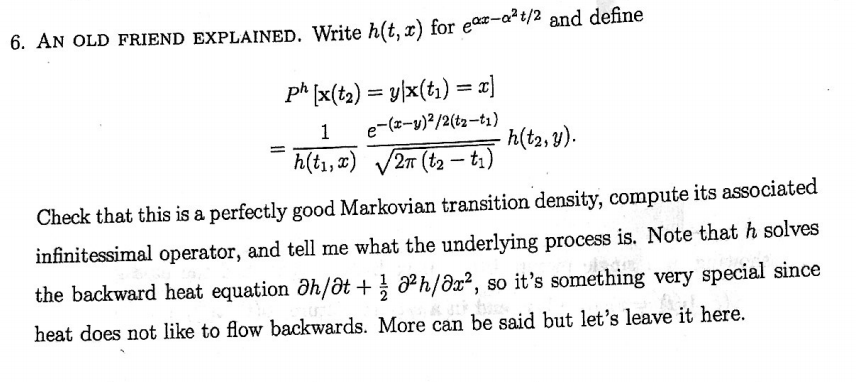
\includegraphics[width=0.7\textwidth]{limthm2-f-p6.png}
\end{figure}
\end{question}
\begin{solution} \hfill \\
\end{solution}
\end{document}
